\documentclass[final]{beamer}
\usepackage[size=custom,width=121.92,height=91.44,scale=1.25]{beamerposter} % 48 x 36 in, landscape
\usetheme{default}\usecolortheme{seagull}
\setbeamertemplate{navigation symbols}{}
\setbeamercolor{block title}{fg=white,bg=black!75}\setbeamercolor{block body}{bg=black!4}
\setbeamertemplate{block begin}{\vskip1ex\begin{beamercolorbox}[ht=3.2ex,dp=1ex,leftskip=1em]{block title}\usebeamerfont*{block title}\insertblocktitle\end{beamercolorbox}\begin{beamercolorbox}[leftskip=1em,rightskip=1em,vmode]{block body}\vskip0.5ex}
\setbeamertemplate{block end}{\vskip0.8ex\end{beamercolorbox}\vskip1ex}
\usepackage{booktabs,graphicx,amsmath}
\graphicspath{{../report/figures/}}
\begin{document}
\begin{frame}[t]
\begin{columns}[t]
\begin{column}{0.98\textwidth}
\begin{center}
{\Huge\bfseries Lost in Pooling: Recovering Small-Signal Evidence Discarded by Frozen Foundation Models}\\[6pt]
{\Large Dhairya Shah \quad Raghav Sarmukaddam \quad Yash Desai \quad Prisha Thakur \quad Ansh Parasher \quad Advait Kale}\\[2pt]
{\large University of Southern California \ \textbullet\ \ CSCI 566, Fall 2026 \ \textbullet\ \ \texttt{github.com/DhairyaShah5/lost-in-pooling}}
\end{center}
\end{column}
\end{columns}
\vspace{6pt}
\begin{columns}[t]
% ---------------------------------------------------------------- column 1
\begin{column}{0.31\textwidth}
\begin{block}{The question}
Frozen vision transformers are deployed as \textbf{one pooled vector} per image (CLS or mean of patch tokens) plus a linear probe. Chest-radiograph evidence says this fails silently on small targets while the same models' patch tokens keep the signal. \textbf{Hypothesis:} the evidence survives the encoder and is lost at \emph{aggregation}.
\end{block}
\begin{block}{One controlled comparison}
On \textbf{identical cached tokens}, swap only the read-out: CLS, mean, max, an \textbf{oracle} that pools the ground-truth region, max-MIL, and a \textbf{gated attention head} trained from image-level labels only. Measure per-class AUROC stratified by the relative size of the largest instance: the \emph{blindness curve}.
\end{block}
\begin{block}{Blindness curve, COCO val2017, DINOv2 ViT-B/14}
\centering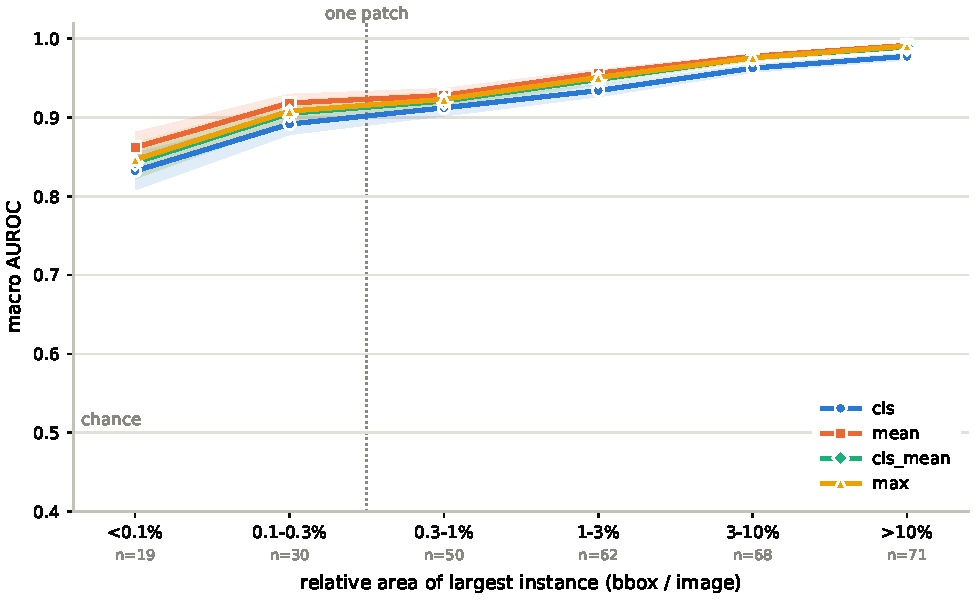
\includegraphics[width=0.95\textwidth]{blindness_curve__dinov2_vitb14_reg__res224.pdf}
\small Global read-outs fall from 0.99 AUROC on large targets to 0.84--0.86 on sub-patch ones; the oracle on the same tokens stays at 0.97. The attention head (no boxes) reaches 0.89 (0.90 multi-scale); mAP 0.73 $\rightarrow$ 0.80 (0.82).
\end{block}
\begin{block}{Same pattern on four backbones}
\centering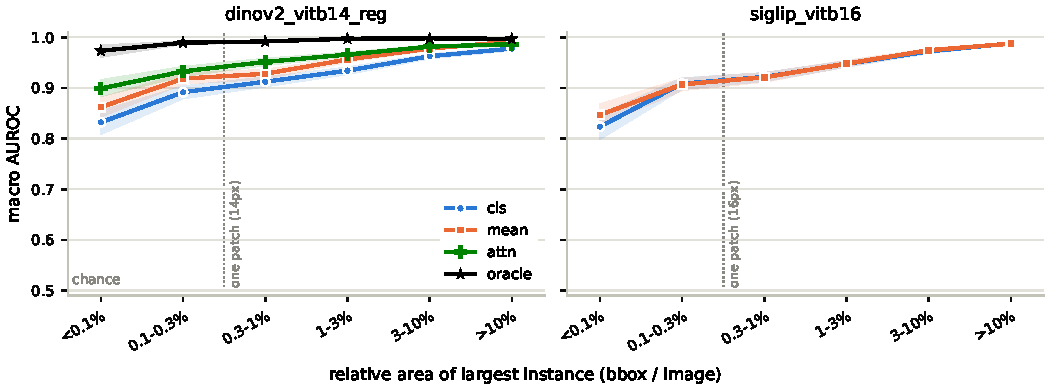
\includegraphics[width=0.98\textwidth]{cross_backbone__res224.pdf}
\small DINOv2, CLIP, SigLIP, DINO ViT-B/16: global read-outs 0.80--0.86 on sub-patch targets, oracles 0.90--0.97, heads in between on every backbone. The 16 px self-supervised model keeps the least small-object evidence, so patch size is not what decides it. Three seeds per read-out.
\end{block}
\end{column}
% ---------------------------------------------------------------- column 2
\begin{column}{0.31\textwidth}
\begin{block}{Where does the head look?}
\centering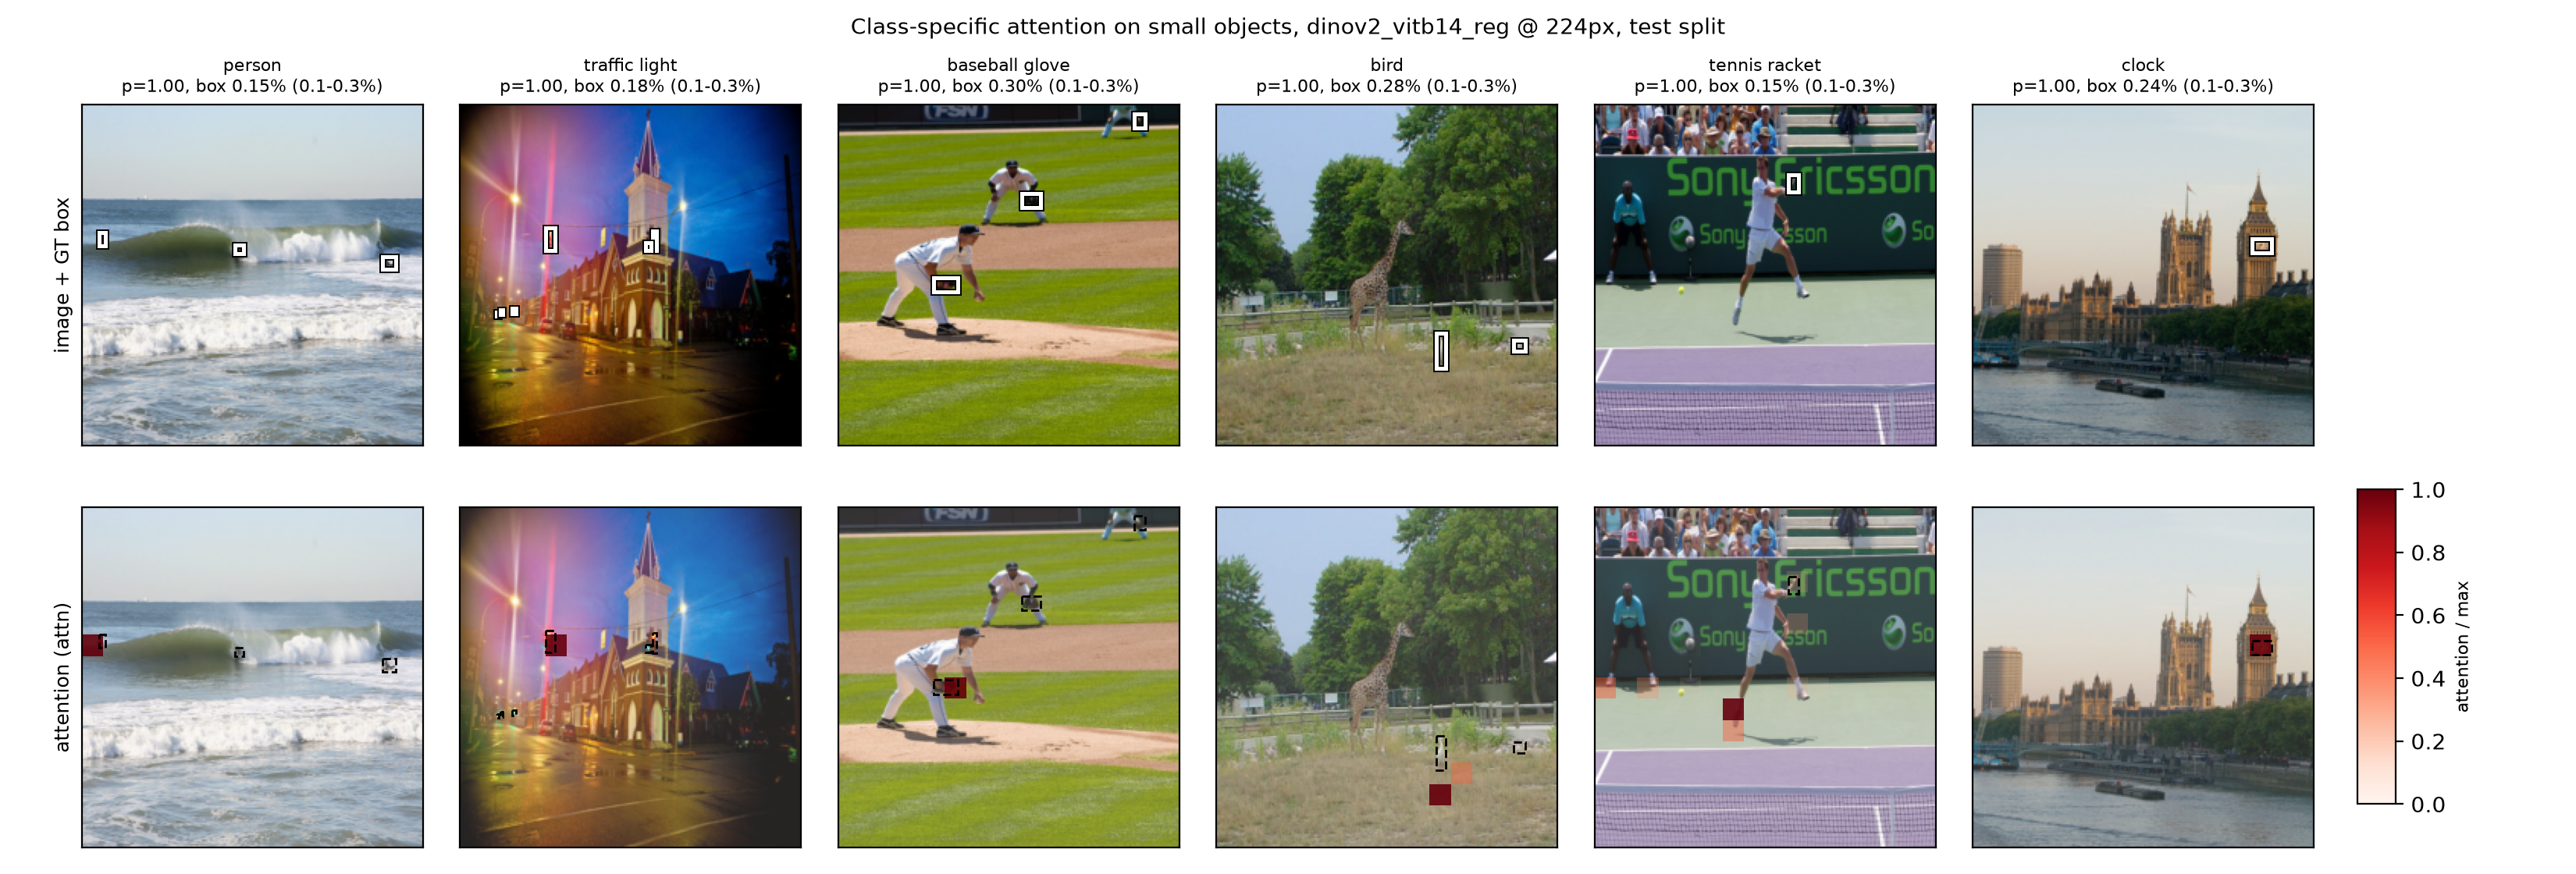
\includegraphics[width=0.98\textwidth]{attention_examples.png}
\small Attention mass inside the ground-truth box is 12 to 24 times chance on small targets. Classes that global pooling loses are those with unpredictable scenes; the per-class oracle gap tracks a context score (Spearman $-0.98$).
\end{block}
\begin{block}{Mechanism: token fraction, not patches}
\centering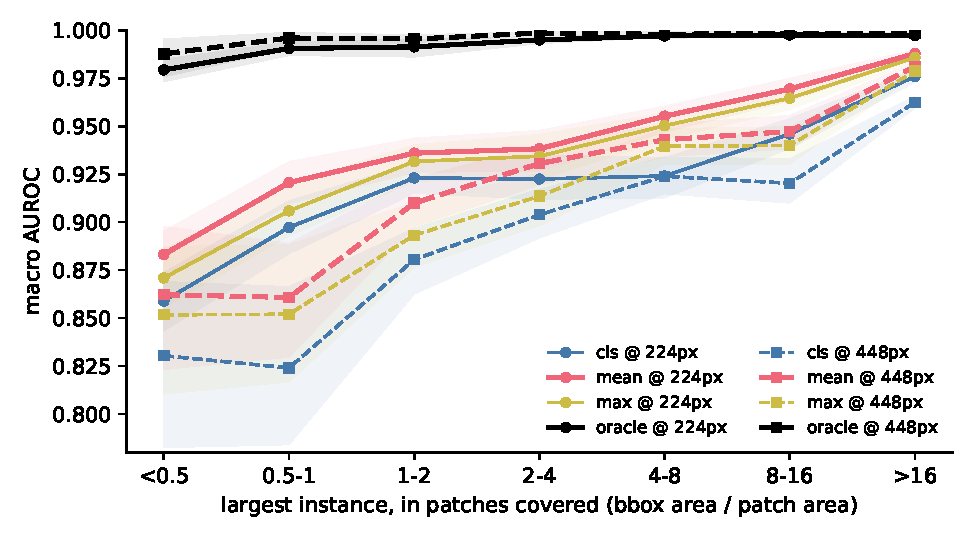
\includegraphics[width=0.85\textwidth]{patch_units__dinov2_vitb14_reg.pdf}
\small 224, 336 and 448 px on the same images. The oracle's curves coincide in \emph{patch} units; global pooling orders itself by \emph{token fraction}: at 448 px a small object is the same share of four times as many tokens, and the probe does not improve.
\end{block}
\begin{block}{Context-only control}
\small Pool only the tokens \emph{outside} the box, with the oracle's own probe. On sub-patch targets it scores \textbf{0.862}, the mean probe's 0.862 exactly (CLIP 0.854 vs 0.838, SigLIP 0.856 vs 0.847): a global read-out on a sub-patch target does no better than a read-out forbidden to see the target. The oracle, which sees only what this control cannot, is 0.973.
\end{block}
\begin{block}{A pre-deployment check}
\centering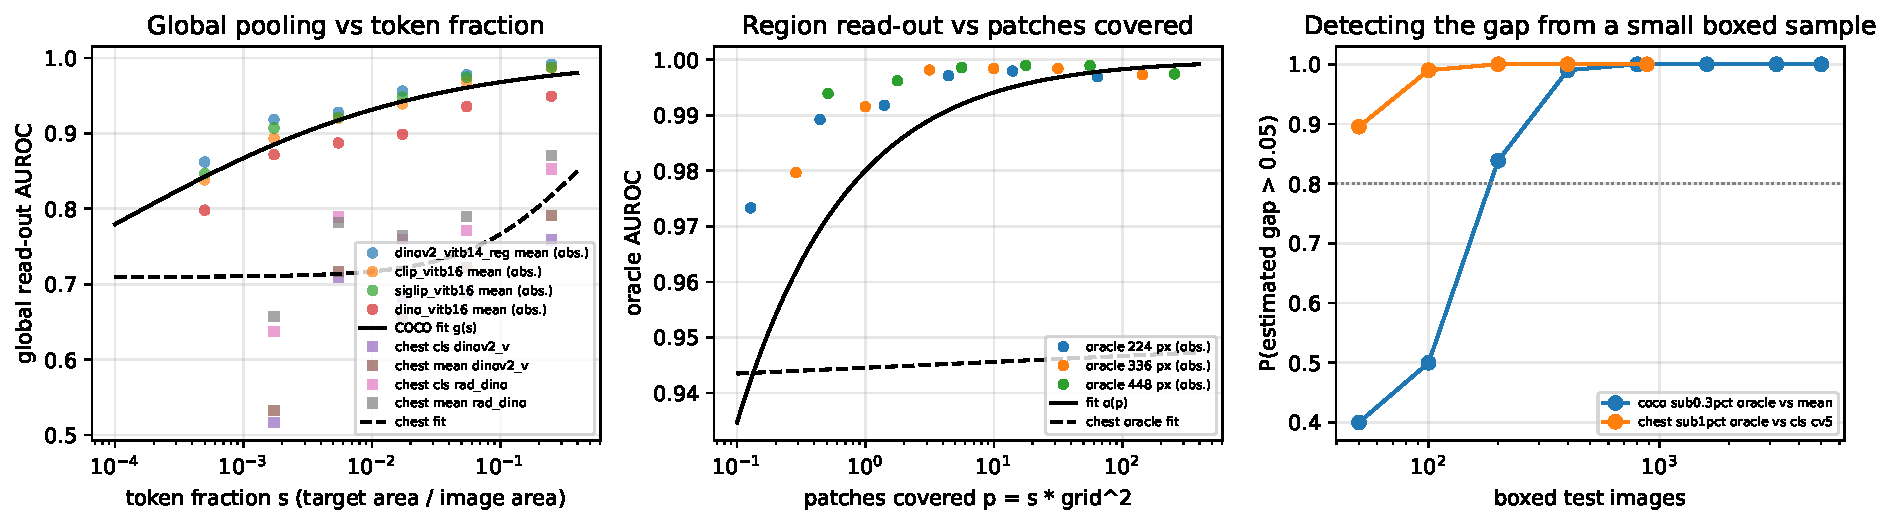
\includegraphics[width=0.98\textwidth]{deploy_check.pdf}
\small Global AUROC is a logistic function of token fraction (within 0.02 across resolutions; leave-one-backbone-out error $\le 0.012$); the radiograph offset is the missing scene prior. 200 boxed images detect the sub-patch gap on COCO, 50 on radiographs. \texttt{python -m lip.eval.deploy\_check --grid 16 --target-frac 0.002}
\end{block}
\end{column}
% ---------------------------------------------------------------- column 3
\begin{column}{0.31\textwidth}
\begin{block}{Radiographs: the cliff reappears}
\centering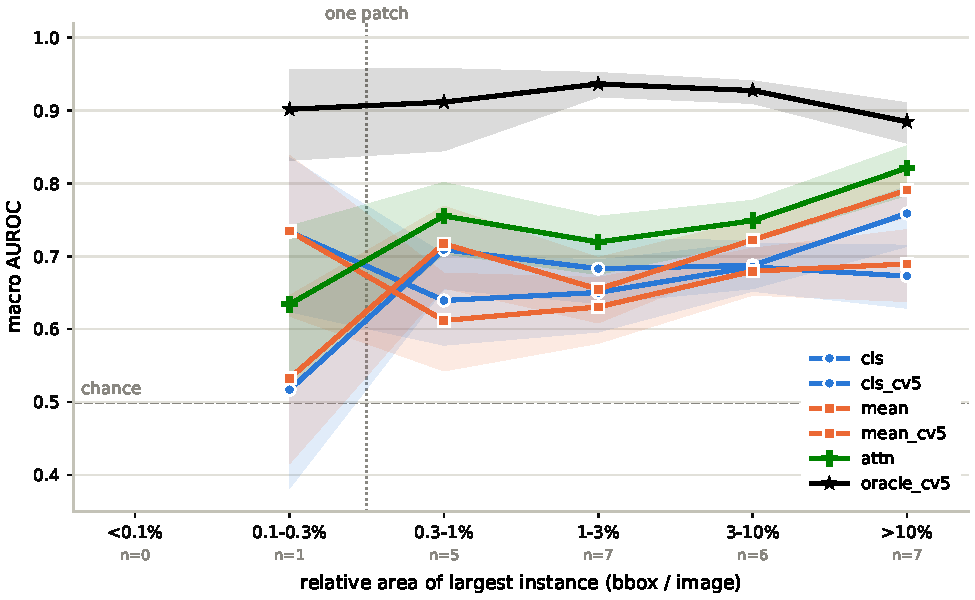
\includegraphics[width=0.8\textwidth]{blindness_curve__dinov2_vitb14_reg__res224_cxr.pdf}
\small NIH ChestX-ray14, 880 boxed images: cross-validated global probes 0.58 vs oracle 0.88--0.94 on the same tokens; image-level probes 0.70; the attention head $0.73\pm0.02$. RAD-DINO raises both sides (oracle 0.95--0.97, probes 0.77) without closing the gap. At 448 px on the full cache the head gains 0.04 ($0.77\pm0.01$), the global probes 0.01. ChestX-Det10 (3,543 images re-annotated by three radiologists, 10 findings): the same cliff on 5.4$\times$ the boxes (global 0.56--0.69 vs oracle 0.91--0.93 under 0.3\% of the frame), and the NIH-trained head transfers (0.74 vs 0.69 for the CLS probe on the shared findings).
\end{block}
\begin{block}{Tiled-teacher distillation}
\small The 224 px head applied to the four quadrants of the 448 px tokens is a teacher that needs no training; a 224 px student trained with its soft targets % TODO(final): distillation numbers
\end{block}
\begin{block}{LUNA16 slices}
\small % TODO(final): LUNA16 figure and numbers
\end{block}
\begin{block}{Take-aways}
\begin{itemize}
\item The loss is at pooling: identical tokens, different read-out, 0.11 AUROC apart on sub-patch targets.
\item Global pooling tracks the \emph{fraction} of tokens a target occupies; resolution alone does not fix it.
\item A head trained from image-level labels recovers part of the gap and looks at the object.
\item Without a scene prior (radiographs) the loss is a cliff; the check above predicts it from target size and token grid.
\end{itemize}
\end{block}
\end{column}
\end{columns}
\end{frame}
\end{document}
